\subsection{Pantalla: Gestionar Programas}
\subsubsection{Objetivo}
	El mapa de navegación se muestra en la Figura~\ref{fig:mapaNavegacionCUG1}

   \begin{figure}[hbpt!]
 		\centering
 			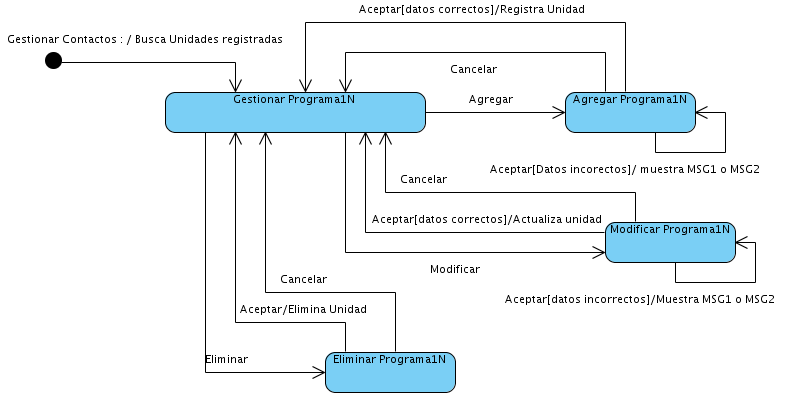
\includegraphics[width=0.8\textwidth]{images/CUG1/mapaNavegacion.png}
 		\caption{Mapa de navegacion para el CU G1 Gestión de Programas.}%
		\label{fig:mapaNavegacionCUG1}
 	\end{figure}

\subsubsection{Objetivo}
	Mostrar la información correspondiente a los Programas a fin de mantener actualizada la información, ver Figura~\ref{IUGestProgramas1N}. Viene de Menú Gestión de Catálogos.

\IUfig[0.8]{CUG1/GestionarPrograma1N.png}{IUGestProgramas1N}{Gestionar Programas.}

\subsubsection{Salidas}

	En esta pantalla se muestran los datos de los Programas registrados en una tabla, ordenados por Nombre de forma ascendente.

\subsubsection{Controles}
\begin{itemize}
 \item \IUbutton{Flecha derecha} Muestra los siguientes n ejes temáticos.
 \item \IUbutton{Flecha izquierda} Muestra los n ejes temáticos anteriores.
\end{itemize}

\subsubsection{Comandos}
\begin{itemize}
 \item \IUbutton{
\includegraphics[scale=0.1]{images/icons/agregar.png}} Esta opción permite registrar un nuevo Programas, al oprimirlo se mostrará la pantalla \IUref{IUAgregarPrograma1N}{Agregar Programa}. Si el Programa se registra correctamente esta aparecerá en la tabla.
 
 \item \IUbutton{
\includegraphics[scale=0.1]{images/icons/editar.png}}: Esta opción permite actualizar los datos de un Programa, tras seleccionar un Programa esta opción lo llevará a la pantalla \IUref{IUModificarPrograma1N}{Modificar Programa}. Si los datos son actualizados correctamente, los cambios se verán en la tabla.

 \item \IUbutton{
\includegraphics[scale=0.1]{images/icons/eliminar.png}}: Esta opción permite eliminar el Programa seleccionado, tras seleccionar un Programa esta opción lo llevará a la pantalla \IUref{IUEliminarPrograma1N}{Eliminar Programa}. Si el Programa se elimina correctamente, esta deberá desaparecer de la tabla.
\end{itemize}

